\documentclass{thesis_proposal}

\title{Improving web accessibility by integrating continuous evaluation to development workflow}
\author{Mariann Tapfer}
\email{tapferm@gmail.com}
 
\begin{document}
\maketitle

% TODO format abstract and keywords/supervisors better
\begin{abstract}
    Improving accessibility is often a struggle, but understanding the extent of the problem and keeping a close eye on it throughout the lifespan of the product could make it more manageable. Continuous integration helps improve and maintain code quality. Could integrating automated accessibility evaluation to the CI pipeline improve the accessibility of the end product in a similar way?
\end{abstract}
\keywords{Web Accessibility, Automatic Evaluation, Continuous Integration, CRM software}
\supervisor{David Jose Ribera Lamas, Mustafa Can Özdemir, Mari-Ell Mets}

\section{Problem Statement}
There is proof that accessibility like user centred design has a profound effect on the quality of products and services and therefore provides a high return on ROI  (Miesenberger et al., 2020) and therefore deserves to be prioritised. 
Developers find it hard to maintain a high level of accessibility over time as it is considered more at the first release of the product (Paternò et al., 2020). Continuous integration is used to speed up development and maintain general code quality (Zhao et al., 2017) and it could also help in maintaining a high level of accessibility by testing the newly added code against predefined accessibility requirements. There is some initial research into the current state of accessibility testing in continuous integration, but it could be improved by doing a case study for an organisation (Sane, 2021).

\section{Research Goal and Research Questions}
This paper aims to map the different automated accessibility evaluation tools, understand their pros and cons and test out one of them on a web based CRM software development process to determine if this practice could help developers in adopting accessibility principles. CRM software was chosen because usability for users with various abilities is an important aspect in a CRM software indicated by mentioning ease of use  and learnability are often in their reviews (23 Best CRM Software and Tools in 2021 | Scoro, 2017) (The Best CRM Software for 2022, n.d.) 

\begin{enumerate}
    % make automated enumeration for RQ1 RQ2..
    \item  RQ1: What kind of errors can automated accessibility testing catch?
    \item RQ2: Can integrating automated testing to a web based CRM-s development pipeline help improve the end products compliance with WCAG standards?
    \item RQ3: Can integrating automated testing to the development pipeline help improve developers awareness and knowledge about accessibility standards?
    \item RQ3: What are the biggest problems in integrating automated accessibility testing software to development workflow?
\end{enumerate}
\section{Methods}
Literature review to map current practices in automating accessibility evaluation focusing on more recent articles and software that could be compatible with the software architecture of the company  later used in the case study.
I will use a user centred research approach where the developers are users to find out what effect could integration of an automated accessibility testing have on the end product and participants knowledge on the subject. I will do some initial testing and prepare examples on what kind of automated testing could be used to detect accessibility problems and the developers from the front-end platform team will decide what kind of approach would be most beneficial and what library or service should be tested. 
After the selection I will configure the testing setup and add some initial tests together with documentation to help understand how to contribute and interpret the results. They will have a chance to improve the testing flow, by tweaking with the settings and adding test cases whenever they feel it's needed.
Pre and post test questionnaire on all developers involved to determine their level of knowledge and attitudes prior to the intervention and see if it is affected. Not all developers will work on the same service or library equally during the research period and some might not even come into contact with it. I will choose the ones that had the most experience and carry out interviews to understand their experience better. 

\section{Research Plan}
Initial research about automated accessibility evaluation tools will be carried out in order to understand the problems and possibilities of this approach and to gain necessary background knowledge to be able to understand and analyse the results of the intervention (see figure 2). 
The case study should be started as soon as possible in order to see its potential impact over time (see figure 3). Everything else is planned around it and everything that is not dependent on the results of the intervention can be done during its progress (see figures 1 and 4). Development of the library or service should not be made more difficult in any way other than drawing attention to any problems with accessibility. 
In addition to articles published in academic journals ones from the most influential web pages and blogs in the field should be included to get most up to date information about the development in the field. 

\begin{figure}[ht!]
    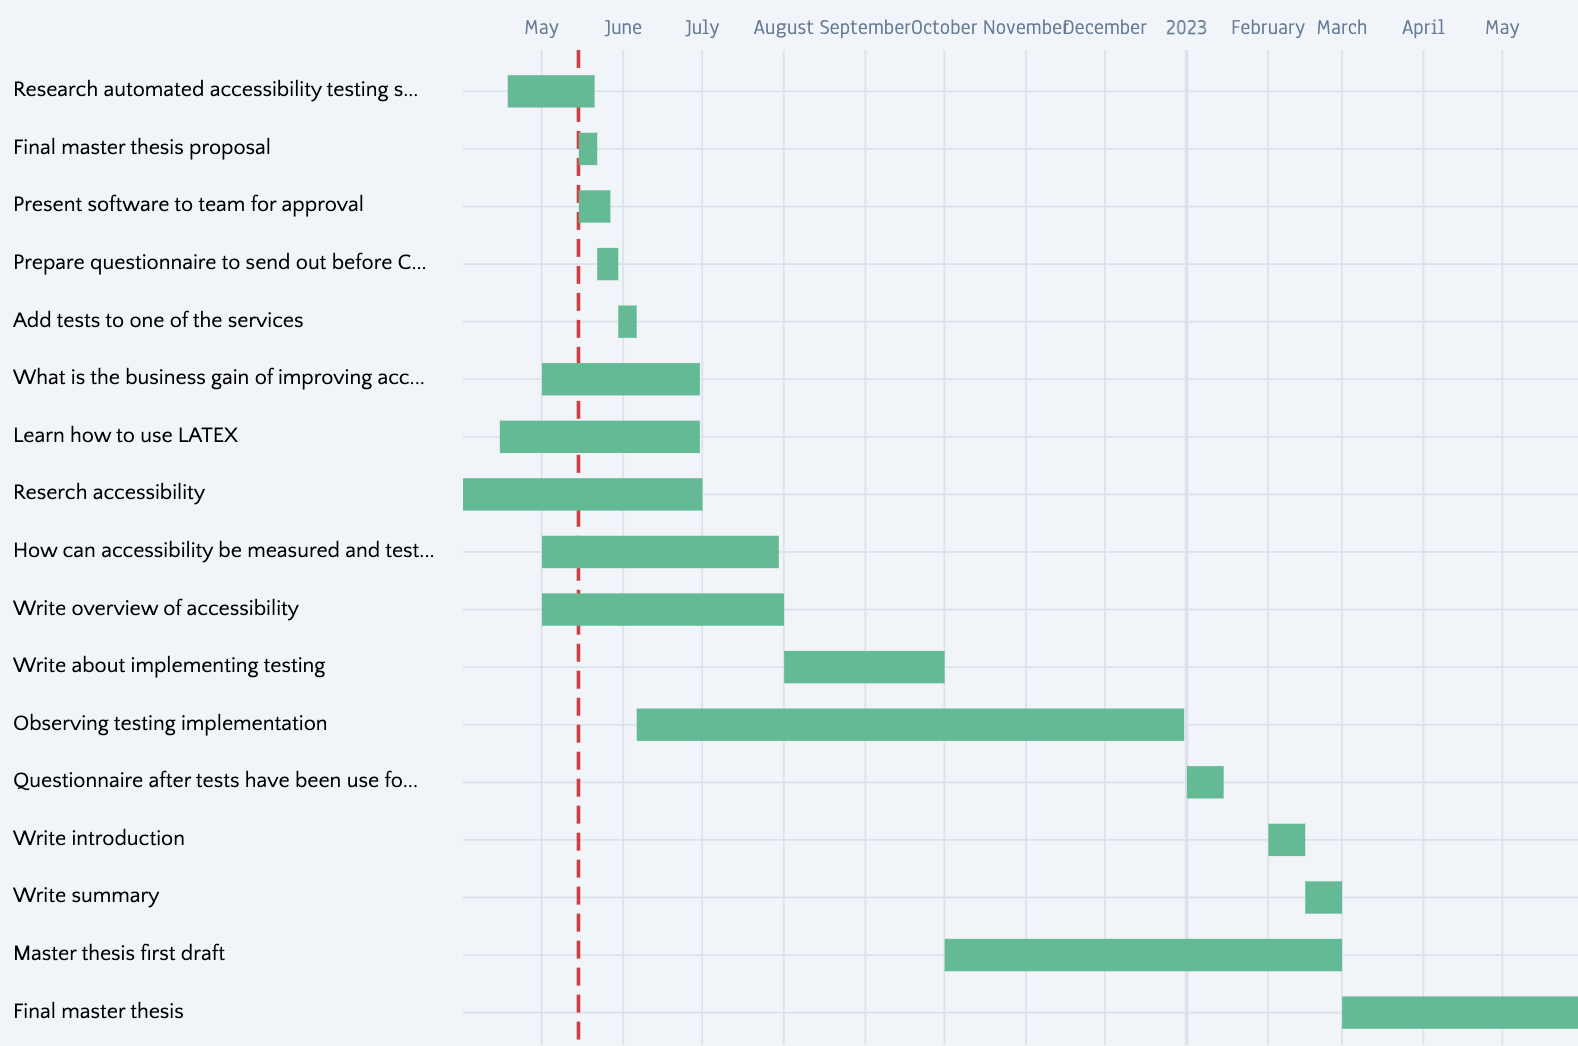
\includegraphics[width=1\textwidth]{img/workplan.png}
    \caption{Master thesis workplan}
\end{figure}
\begin{figure}[ht!]
    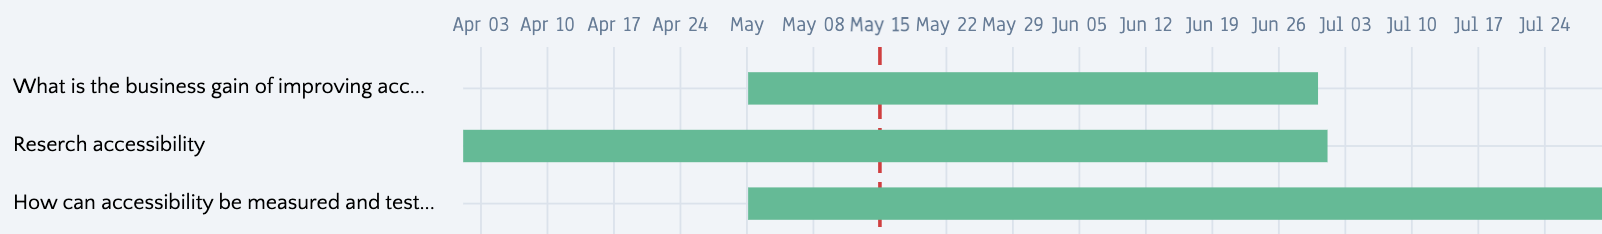
\includegraphics[width=1\textwidth]{img/research_accessibility.png}
    \caption{Accessibility research plan}
\end{figure}
\begin{figure}[ht!]
    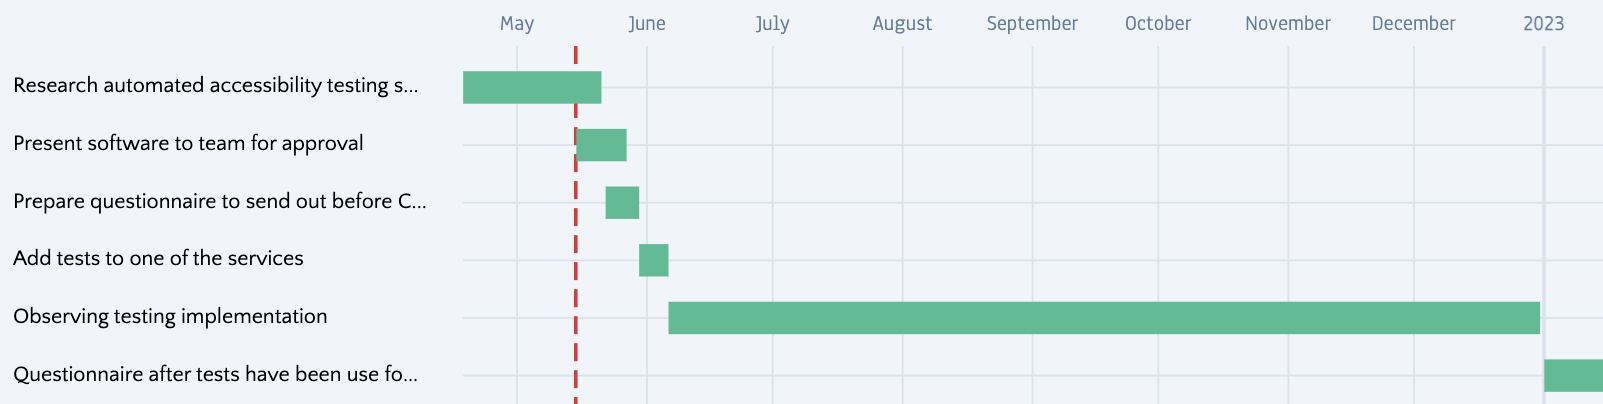
\includegraphics[width=1\textwidth]{img/case_study.png}
    \caption{Case study work plan}
\end{figure}
\begin{figure}[ht!]
    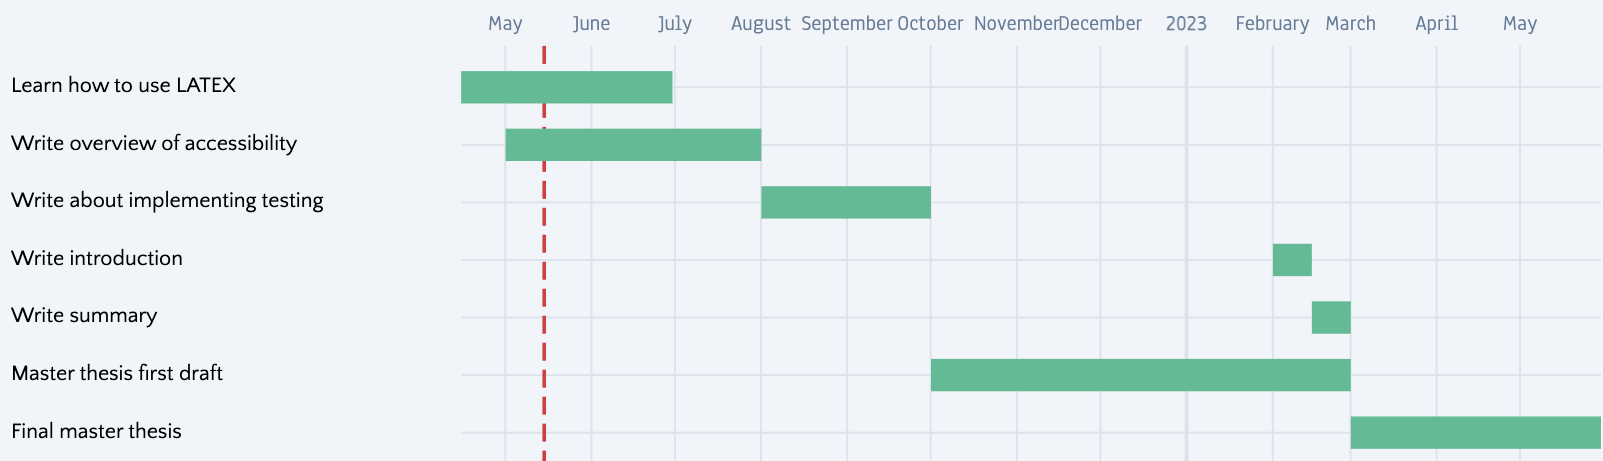
\includegraphics[width=1\textwidth]{img/thesis_writing.png}
    \caption{Thesis writing plan}
\end{figure}

\section{References}
% TODO: add references

\end{document}